\documentclass[a4paper]{article} 
\addtolength{\hoffset}{-2.25cm}
\addtolength{\textwidth}{4.5cm}
\addtolength{\voffset}{-3.25cm}
\addtolength{\textheight}{5cm}
\setlength{\parskip}{0pt}
\setlength{\parindent}{0in}

%----------------------------------------------------------------------------------------
%	PACKAGES AND OTHER DOCUMENT CONFIGURATIONS
%----------------------------------------------------------------------------------------

\usepackage{blindtext} % Package to generate dummy text
\usepackage{charter} % Use the Charter font
\usepackage[utf8]{inputenc} % Use UTF-8 encoding
\usepackage{microtype} % Slightly tweak font spacing for aesthetics
\usepackage[english, ngerman]{babel} % Language hyphenation and typographical rules
\usepackage{amsthm, amsmath, amssymb} % Mathematical typesetting
\usepackage{float} % Improved interface for floating objects
\usepackage[final, colorlinks = true, 
            linkcolor = black, 
            citecolor = black]{hyperref} % For hyperlinks in the PDF
\usepackage{graphicx, multicol} % Enhanced support for graphics
\usepackage{xcolor} % Driver-independent color extensions
\usepackage{marvosym, wasysym} % More symbols
\usepackage{rotating} % Rotation tools
\usepackage{censor} % Facilities for controlling restricted text
\usepackage{listings, style/lstlisting} % Environment for non-formatted code, !uses style file!
\usepackage{pseudocode} % Environment for specifying algorithms in a natural way
\usepackage{style/avm} % Environment for f-structures, !uses style file!
\usepackage{booktabs} % Enhances quality of tables
\usepackage{tikz-qtree} % Easy tree drawing tool
\tikzset{every tree node/.style={align=center,anchor=north},
         level distance=2cm} % Configuration for q-trees
\usepackage{style/btree} % Configuration for b-trees and b+-trees, !uses style file!
\usepackage[backend=biber,style=numeric,
            sorting=nyt]{biblatex} % Complete reimplementation of bibliographic facilities
\addbibresource{ecl.bib}
\usepackage{csquotes} % Context sensitive quotation facilities
\usepackage[yyyymmdd]{datetime} % Uses YEAR-MONTH-DAY format for dates
\renewcommand{\dateseparator}{-} % Sets dateseparator to '-'
\usepackage{fancyhdr} % Headers and footers
\pagestyle{fancy} % All pages have headers and footers
\fancyhead{}\renewcommand{\headrulewidth}{0pt} % Blank out the default header
\fancyfoot[L]{} % Custom footer text
\fancyfoot[C]{} % Custom footer text
\fancyfoot[R]{\thepage} % Custom footer text
\newcommand{\note}[1]{\marginpar{\scriptsize \textcolor{red}{#1}}} % Enables comments in red on margin

%----------------------------------------------------------------------------------------

% \usepackage{bm}
% \usepackage{amsmath}
% \usepackage{graphicx}

\graphicspath{{images/}}
\begin{document}

%-------------------------------
%	TITLE SECTION
%-------------------------------

\fancyhead[C]{}
\hrule \medskip % Upper rule
\begin{minipage}{0.295\textwidth} 
\raggedright
\footnotesize
SHRUTI RAO \hfill\\   
2636454 \hfill\\
s2.rao@student.vu.nl
\end{minipage}
\begin{minipage}{0.4\textwidth} 
\centering 
\large 
Homework Assignment 5\\ 
\normalsize 
Machine Learning 1, 19/20\\ 
\end{minipage}
\begin{minipage}{0.295\textwidth} 
\raggedleft
\today\hfill\\
\end{minipage}
\medskip\hrule 
\bigskip

%-------------------------------
%	CONTENTS
%-------------------------------

\section*{A K Sided Die}
\subsection*{1}
The log posterior is given by:
\begin{align*}
    p(\pmb{\theta}|\mathcal{D}) \propto p(\mathcal{D}|\pmb{\theta})p(\pmb{\theta}) &= \prod_{k=1}\pmb{\theta}_{k}^{N_{k} + \alpha_{k} -1} \\
\end{align*}{}

Then, its log is given by:
\begin{align*}
    \ln{p(\pmb{\theta}|\mathcal{D})} &= \ln{\prod_{k=1}\pmb{\theta}_{k}^{N_{k} + \alpha_{k} -1}} \\
    &= \sum_{k}\ln{\pmb{\theta}_{k}^{N_{k} + \alpha_{k} -1}}\\
    &= \sum_{k}(N_{k} + \alpha_{k} -1)\ln{\pmb{\theta}_{k}}
\end{align*}

\subsection*{2}
The constraints are:
\begin{itemize}
    \item $\sum_{k=1}^{K}\pmb{\theta}_{k}=1$
    \item $\sum_{k=1}^{K}\pmb{\theta}_{k} \geq 0$
\end{itemize}

The Lagrangian is then given by:
\begin{align*}
    \mathcal{L}(\pmb{\theta}, \lambda, \pmb{\mu}) &= \sum_{k}(N_{k} + \alpha_{k} -1)\ln{\pmb{\theta}_{k}} + \lambda(\sum_{k=1}^{K}\pmb{\theta}_{k} - 1) + \sum_{k=1}^{K}(\mu_{k}\pmb{\theta}_{k})
\end{align*}

\subsection*{3}
The KKT conditions are:
\begin{enumerate}
    \item $\theta_{k}-1 = 0 \ \forall k$
    \item $\theta_{k} \geq 0 \ \forall k$
    \item $\mu_{k}\theta_{k} = 0 \ \forall k$
    \item $\lambda \geq 0 $
    \item $ \mu_{k} \geq 0 \ \forall k$
\end{enumerate}

\subsection*{4}
We need to now find $\pmb{\theta}_{MAP}$:

\begin{align*}
    \frac{\partial \mathcal{L}(\pmb{\theta}, \lambda, \pmb{\mu})}{\partial \pmb{\theta}} &= \frac{\partial \sum_{i=1}^{K}(N_{k} + \alpha_{k} -1)\ln{\pmb{\theta}_{k}} + \lambda(\sum_{i=1}^{K}\pmb{\theta}_{k} - 1) + \sum_{i=1}^{K}(\pmb{\mu}_{k}\pmb{\theta}_{k})}{\partial \pmb{\theta}} \\
    0 &=\frac{\sum_{i=1}^{K}(N_{k} + \alpha_{k} -1)}{\pmb{\theta}_{k}} + \lambda + \sum_{i=1}^{K}\pmb{\mu}_{k}\\
    0 &= \frac{\sum_{i=1}^{K}N_{k} + \sum_{i=1}^{K}\alpha_{k} -\sum_{i=1}^{K}1}{\pmb{\theta}_{k}} + \lambda + \sum_{i=1}^{K}\pmb{\mu}_{k}\\
    0 &= N_{K} + \alpha_{K} - K + \pmb{\theta}_{k}\lambda + \pmb{\theta}_{k}\sum_{i=1}^{K}\pmb{\mu}_{k} \\
    \pmb{\theta}_{k}\lambda + \pmb{\theta}_{k}\sum_{i=1}^{K}\pmb{\mu}_{k} &=  K - N_{K} - \alpha_{K}\\
    \pmb{\theta}_{k} [\lambda + \sum_{i=1}^{K}\pmb{\mu}_{k}] &= K - N_{K} - \alpha_{K}\\
    \pmb{\theta}_{MAP} = \frac{K - N_{K} - \alpha_{K}}{\lambda + \sum_{i=1}^{K}\pmb{\mu}_{k}}
\end{align*}
\bigskip

\section*{Maximum Margin Classifier}
\subsection*{1}
The Lagrangian multipliers are:
\begin{itemize}
    \item ${\lambda_{n}} $
    \item ${\mu_{n}}$
\end{itemize}

The constraints are:
\begin{itemize}
    \item $t_{n}(\beta||x_{n}|| - R) \geq 1 - \xi_{n}$
    \item $\xi_{n} \geq 0$
\end{itemize}

Combining the multipliers and constraints together, we get the primal Lagrangian as:
\begin{align*}
    \mathcal{L}(R, \beta, \pmb{\xi}) &= \frac{1}{2}\beta^{2} + C\sum_{n=1}^{N}\pmb{\xi}_{n} - \sum_{n=1}^{N}\lambda_{n}[t_{n}(\beta||x_{n}|| - R) - 1 + \pmb{\xi}_{n}] - \sum_{n=1}^{K}\mu_{n}\pmb{\xi}_{n}\\
\end{align*}

\subsection*{2}
The derivatives for $\beta, R, \xi$ can be calculated first:

\subsubsection*{$\beta$:}
\begin{align*}
    \frac{\partial \mathcal{L}}{\partial \beta} &= \beta - \sum_{i=1}^{N}\lambda_{n}t_{n}||x_{n}|| = 0 \\
    \beta &= \sum_{n=1}^{N}\lambda_{n}t_{n}||x_{n}||
\end{align*}

\subsubsection*{$R$:}
\begin{align*}
    \frac{\partial \mathcal{L}}{\partial R} &= \sum_{n=1}^{N}\lambda_{n}t_{n} = 0
\end{align*}

\subsubsection*{$\pmb{\xi}$:}
\begin{align*}
    \frac{\partial \mathcal{L}}{\partial \pmb{\xi}} &= C - \lambda_{n} - \mu_{n}\\
\end{align*}

There in 6 KKT conditions,  given by:
\begin{enumerate}
    \item $t_{n}(\beta||x_{n}|| - R) - 1 + \pmb{\xi}_{n} \geq 0  \ \forall n$
    \item $\pmb{\xi}_{n} \geq 0 \ \forall n$
    \item $\lambda_{n}  \geq \ \forall n$
    \item $ \mu_{n} \geq 0  \ \forall n$
    \item $\lambda_{n}[t_{n}(\beta||x_{n}|| - R) - 1 + \pmb{\xi}_{n}] = 0  \ \forall n$
    \item $\mu_{n}\pmb{\xi}_{n} = 0 \ \forall n$
\end{enumerate}

\subsection*{3}
The dual Lagrangian can be obtained by eliminating the primals ${\beta, R, \xi_{1},..,\xi_{k}}$:

\begin{align*}
    \mathcal{L}(R, \beta, \pmb{\xi}) &= \frac{1}{2}\beta^{2} + C\sum_{n=1}^{N}\pmb{\xi}_{n} - \sum_{n=1}^{N}\lambda_{n}[t_{n}(\beta||x_{n}|| - R) - 1 + \pmb{\xi}_{n}] - \sum_{n=1}^{K}\mu_{n}\pmb{\xi}_{n}\\
    &= \frac{1}{2}\beta^{2} + C\sum_{n=1}^{N}\pmb{\xi}_{n} - 
    \sum_{n=1}^{N}[\lambda_{n}t_{n}\beta||x_{n}|| - \lambda_{n}t_{n}R - \lambda_{n} + \lambda_{n}\pmb{\xi}_{n}] - \sum_{n=1}^{K}\mu_{n}\pmb{\xi}_{n}\\
    &= \frac{1}{2}\left [\sum_{n=1}^{N}\lambda_{n}t_{n}||x_{n}|| \right]^{2} + (\mu_{n} + \lambda_{n})\sum_{n=1}^{N}\pmb{\xi}_{n} - \sum_{n=1}^{N}[\lambda_{n}t_{n}\beta||x_{n}|| - 0 - \lambda_{n} + \lambda_{n}\pmb{\xi}_{n}] - \sum_{n=1}^{K}\mu_{n}\pmb{\xi}_{n}\\
    &= \frac{1}{2}\left [\sum_{n=1}^{N}\lambda_{n}t_{n}||x_{n}|| \right]^{2} +  \mu_{n}\sum_{n=1}^{N}\pmb{\xi}_{n} + \lambda_{n}\sum_{n=1}^{N}\pmb{\xi}_{n} - \sum_{n=1}^{N}\lambda_{n}t_{n}\beta||x_{n}|| + \sum_{n=1}^{N}\lambda_{n} - \sum_{n=1}^{N}\lambda_{n}\pmb{\xi}_{n} - \sum_{n=1}^{K}\mu_{n}\pmb{\xi}_{n}\\
    &= \left [\sum_{n=1}^{N}\lambda_{n}t_{n}||x_{n}|| \right]^{2}  - \sum_{n=1}^{N}\lambda_{n}t_{n}\beta||x_{n}|| + \sum_{n=1}^{N}\lambda_{n}\\
    &= \frac{1}{2}\sum_{n=1}^{N}\sum_{j=1}^{N}\lambda_{n}\lambda_{j}t_{n}t_{j}||x_{n}|| \ ||x_{j}|| - \sum_{n=1}^{N}\sum_{j=1}^{N}\lambda_{n}\lambda_{j}t_{n}t_{j}||x_{n}|| \ ||x_{j}|| + \sum_{n=1}^{N}\lambda_{n}\\
    &= \sum_{n=1}^{N}\lambda_{n} - \frac{1}{2} \sum_{n=1}^{N}\sum_{j=1}^{N}\lambda_{n}\lambda_{j}t_{n}t_{j}||x_{n}|| \ ||x_{j}||
\end{align*}

The dual problem is:
$argmax \ \lambda_{n} \sum_{n=1}^{N}\lambda_{n} - \frac{1}{2} \sum_{n=1}^{N}\sum_{j=1}^{N}\lambda_{n}\lambda_{j}t_{n}t_{j}||x_{n}|| \ ||x_{j}||$ 

The constraints are:
\begin{itemize}
    \item $\lambda_{n} \geq 0 \ \forall n$
    \item $\sum_{n=1}t_{n}\lambda_{n} = 0 \ \forall n$
\end{itemize}


\subsection*{4}
The explicit form of $k(x, x') = f(x)f(x')$

\begin{align*}
    k(x_{n}, x_{j}) &= ||x_{n}||\ ||x_{j}||\\
    &= x_{n}^{T}x_{n} \ x^{T}_{j}x_{j}
\end{align*}

\subsection*{5}
$\lambda_{n}[t_{n}(\beta||x_{n}|| - R) - 1 + \pmb{\xi}_{n}] = 0  \ \forall n$ thus $[t_{n}(\beta||x_{n}|| - R) - 1 + \pmb{\xi}_{n}] = 0$ or $\lambda_{n} = 0$. However, from the given condition, $\lambda_{n}$ is greater than zero and less than C. Hence, it cannot equal 0. Moreover, if $\lambda$ did equal 0, it would mean that the constraint is already satisfied since the point is already inside the boundary. 

\subsection*{6}
\begin{align}
    y(x, \beta) &= a^{T}k \\
    y(x^{*})&= \beta||x^{*}|| - R \\
    \text{Since } \beta &= \sum_{n=1}^{N}\lambda_{n}t_{n}||x_{n}|| \\
    y(x^{*}) &= \sum_{n=1}^{N}\lambda_{n}t_{n}||x_{n}||||x^{*}|| - R \\
    &= \sum_{n=1}^{N}\lambda_{n}t_{n}k(x_{n},x^{*}) - R  \text{  \ \ \ \  [from 5.]}
\end{align}

\subsection*{7}

For $\lambda_{n}[t_{n}(\beta||x_{n}|| - R) - 1 + \pmb{\xi}_{n}] = 0  \ \forall n$ \\
\begin{itemize}
    \item if $t_{n}(\beta||x_{n}|| < 0$ then $\lambda_{n} = 0$. \\ Using this and the derivative for $\xi$ (Section 2.2): \\
    $C - \lambda_{n} - \mu_{n} => \\
    C =  \mu_{n} $ (point inside boundary)
    \item if $t_{n}(\beta||x_{n}|| = 0$ then $\lambda_{n} \geq 0$ (point outside or on boundary)
\end{itemize}

For $\mu_{n}\pmb{\xi}_{n} = 0 \ \forall n$:\\
\begin{itemize}
    \item if $\mu_{n} > 0$ then $ \xi_{n}  = 0$ (inside or on boundary)
    \item if $\mu_{n} = 0$ then $ \xi_{n}  \geq 0$ (outside  boundary)
\end{itemize}


\subsection*{8}
When $0 < \lambda_{n} < C$ then $x_{n}$ must be on the boundary.\\
When $\lambda_{n} = 0$, then $x_{n}$ must be inside or on the boundary.\\
When $\lambda_{n} = C$, then $x_{n}$ must be on or outside the boundary.\\

\begin{align*}
    u_{n}^{*} = C - \lambda_{n}
\end{align*}

\subsubsection*{$\beta$:}
\begin{align*}
    \beta^{*} &= \sum_{n=1}^{N}\lambda_{n}t_{n}||x_{n}||
\end{align*}

\subsubsection*{R}
\begin{align*}
   \lambda_{n}[t_{n}(\beta||x_{n}|| - R) - 1 + \pmb{\xi}_{n}] &= 0 \\
   \text{When } \lambda_{n} = 0: \\
   t_{n}\beta||x_{n}|| - t_{n}R - 1 + \pmb{\xi}_{n} &= 0 \\
   t_{n}R = t_{n}\beta||x_{n}|| - 1 + \pmb{\xi}_{n}   \\
   R^{*} = \beta^{*}||x_{n}|| - \frac{1}{t_{n}} + \frac{\pmb{\xi}_{n}}{t_{n}}
\end{align*}

\subsubsection*{$\xi$:}
\[
\begin{cases}
    1 - t_{n}(\beta^{*}||x_{n}|| - R) & \text{for }\lambda_{n} = C \\
    0 & \text{for }\lambda_{n} = 0\\
\end{cases}
\]
 
\subsection*{9}
Yes the decision boundary would be different since the kernel would be more complex and draw with greater precision. 

\begin{figure}[h]
    \centering
    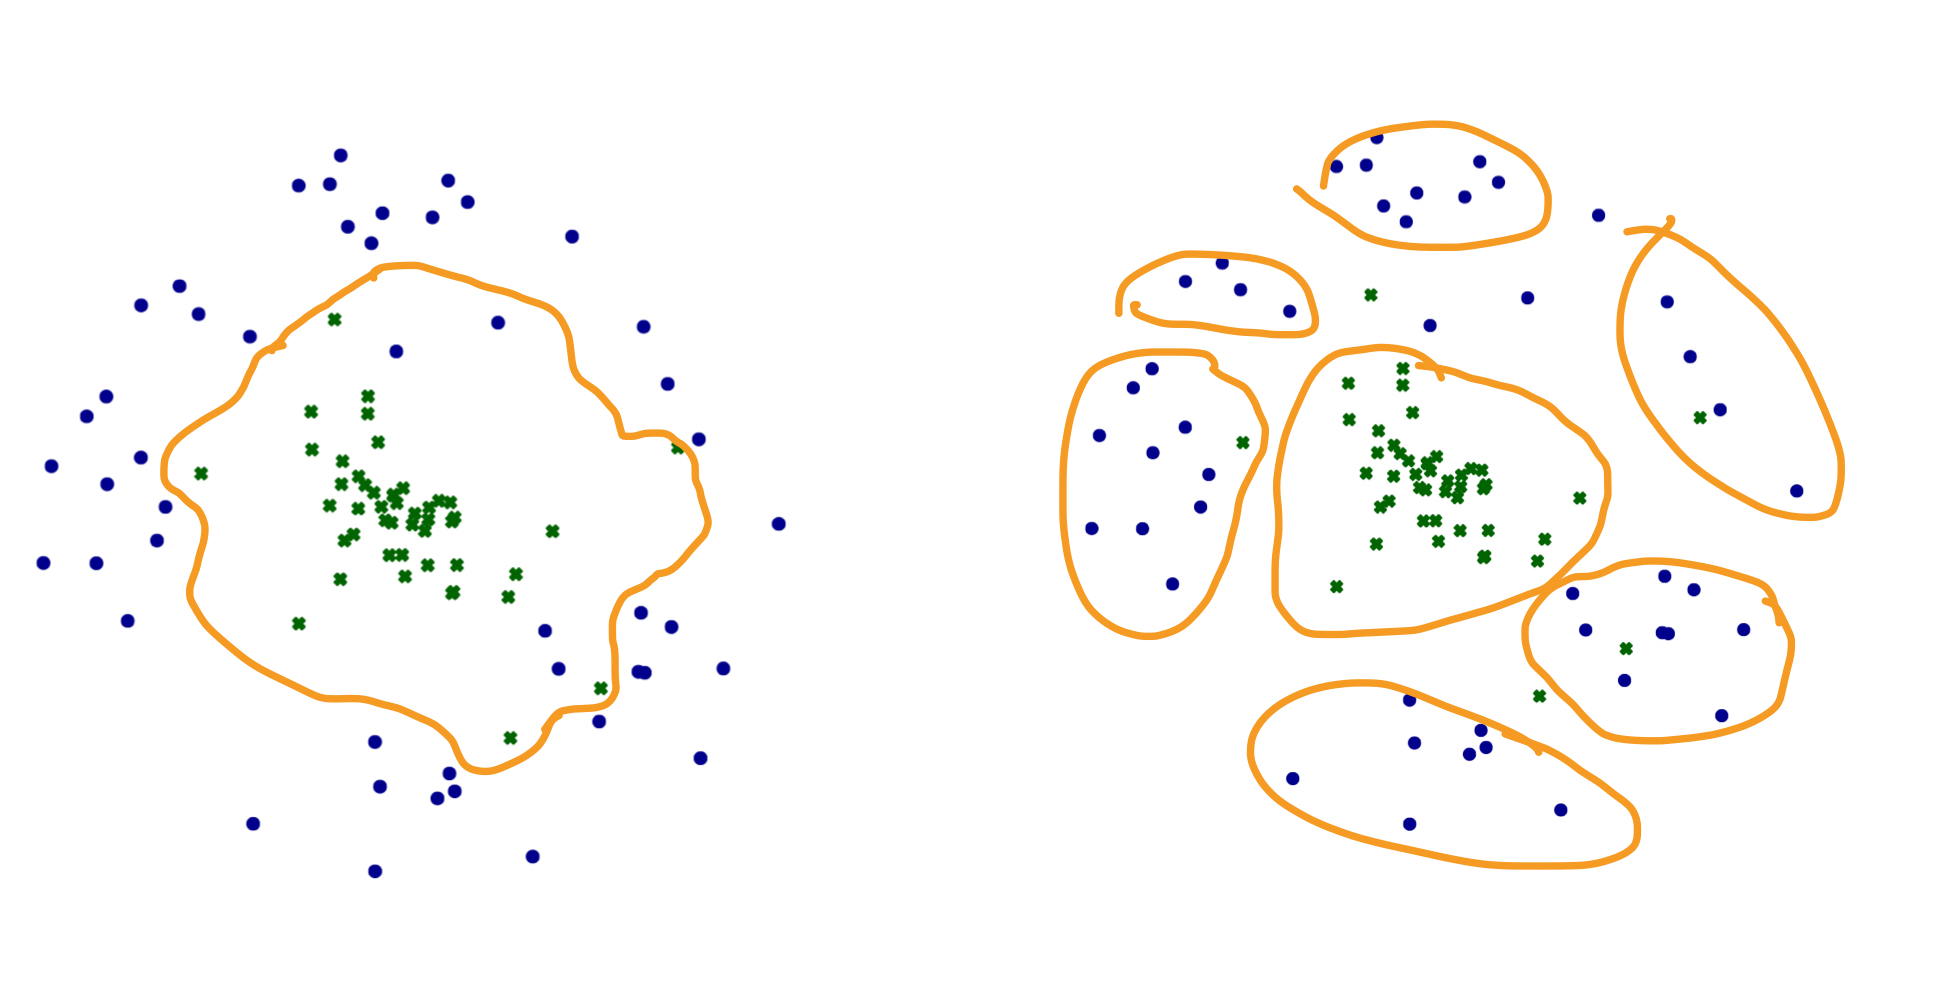
\includegraphics[width=0.45\textwidth]{IMG_A18C3AA43921-1.jpeg}
    \caption{Data with Radial Basis Function Boundary (Yellow)}
    \label{fig:my_label}
\end{figure}

\end{document}
